\documentclass{standalone}
\usepackage{tikz}
\usetikzlibrary{arrows.meta}

\begin{document}
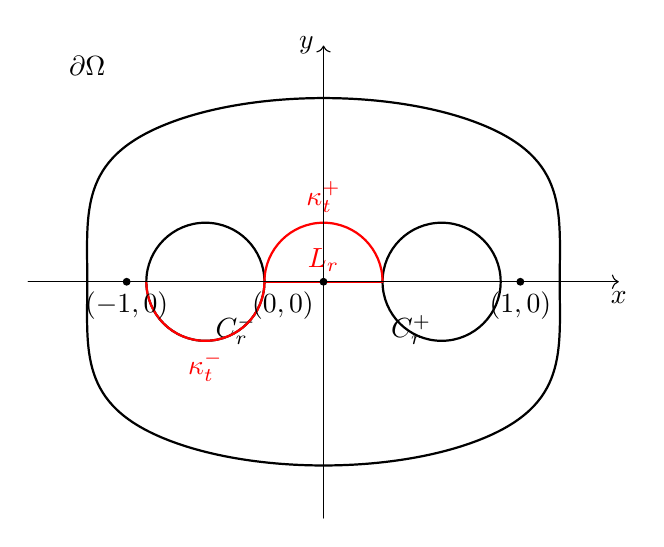
\begin{tikzpicture}[line cap=round, line join=round, scale=2.5]
    % Draw the boundary curve
    \draw[thick] plot[smooth cycle, tension=0.8] coordinates {(-1.2, 0) (-0.8, 0.8) (0.8, 0.8) (1.2, 0) (0.8, -0.8) (-0.8, -0.8)};
    
    % Draw the two circles
    \draw[thick] (0.6,0) circle (0.3) node[below left, yshift=-0.3cm] {\(C_r^+\)};
    \draw[thick] (-0.6,0) circle (0.3) node[below right, yshift=-0.3cm] {\(C_r^-\)};
    
    % Draw the red line connecting the two circles
    \draw[red, thick] (0.3,0) -- (-0.3,0) node[midway, above] {\(L_r\)};
    
    % Label the arcs
    \draw[red, thick] (0.3,0) arc(0:180:0.3) node[pos=0.5, above] {\(\kappa_t^+\)};
    \draw[red, thick] (-0.9,0) arc(180:360:0.3) node[pos=0.5, below] {\(\kappa_t^-\)};
    
    % Axes
    \draw[->] (-1.5,0) -- (1.5,0) node[below] {\(x\)};
    \draw[->] (0,-1.2) -- (0,1.2) node[left] {\(y\)};
    
    % Important points on the x-axis
    \fill (1,0) circle (0.02) node[below] {\((1,0)\)};
    \fill (-1,0) circle (0.02) node[below] {\((-1,0)\)};
    \fill (0,0) circle (0.02) node[below left] {\((0,0)\)};
    
    % Boundary label
    \node[above] at (-1.2,1) {\(\partial\Omega\)};
\end{tikzpicture}
\end{document}